% VLDB template version of 2020-08-03 enhances the ACM template, version 1.7.0:
% https://www.acm.org/publications/proceedings-template
% The ACM Latex guide provides further information about the ACM template
%\usepackage{caption}
%\usepackage{subfigure}
\documentclass[sigconf, nonacm]{acmart}
\usepackage{subfigure}
\usepackage{minted}
\usepackage{pdfpages}

\usepackage{listings}
\usepackage{xcolor}
%% The following content must be adapted for the final version
% paper-specific
\newcommand\vldbdoi{XX.XX/XXX.XX}
\newcommand\vldbpages{XXX-XXX}
% issue-specific
\newcommand\vldbvolume{14}
\newcommand\vldbissue{1}
\newcommand\vldbyear{2020}
% should be fine as it is
\newcommand\vldbauthors{\authors}
\newcommand\vldbtitle{\shorttitle} 
% leave empty if no availability url should be set
\newcommand\vldbavailabilityurl{http://vldb.org/pvldb/format_vol14.html}
% whether page numbers should be shown or not, use 'plain' for review versions, 'empty' for camera ready
\newcommand\vldbpagestyle{plain} 



\begin{document}
\title{CLIC: A Cloud-Native Framework for Building Cross-Platform Data Analytics Workflows}


% The "author" command and its associated commands are used to define the authors and their affiliations.
\author{Qixiang Chen, Kai Zhang, Qinghua Du, Fengyi Liu, Zhijun Chen, Xiaomin Xu, Yinan Jing, Zhenying He, X. Sean Wang}
\affiliation{
 \institution{Fudan University}
}
\email{{qxchen19, zhangk, qhdu19, zjchen20, xiaominxu20, jingyn, zhenying, xywangCS}@fudan.edu.cn}


%%
%% The abstract is a short summary of the work to be presented in the
%% article.
\begin{abstract}
With the ever-increasing data volume and business logic complexity, a modern data science application is generally built as a workflow consisting of multiple tasks, which are deployed on different data processing platforms for either specific functionalities or higher performance. With the high scalability and availability, cloud computing is promising for building such data science applications. However, existing cross-platform frameworks are not designed for cloud and cannot exploit its advantages.

This paper proposes CLIC, a cloud-native framework for cross-platform data science applications. By deploying workflows with a cloud-native architecture and assigning tasks to the most appropriate computing platforms via a deep learning model, CLIC can enhance the performance of modern data science applications while reducing the development and deployment efforts. Moreover, CLIC also demonstrates high extensibility in coping with various scenarios by easily integrating new platforms of different programming languages and paradigms.
\end{abstract}

\maketitle

%%% do not modify the following VLDB block %%
%%% VLDB block start %%%
\iffalse
\pagestyle{\vldbpagestyle}
\begingroup\small\noindent\raggedright\textbf{PVLDB Reference Format:}\\
\vldbauthors. \vldbtitle. PVLDB, \vldbvolume(\vldbissue): \vldbpages, \vldbyear.\\
\href{https://doi.org/\vldbdoi}{doi:\vldbdoi}
\endgroup
\begingroup
\renewcommand\thefootnote{}\footnote{\noindent
This work is licensed under the Creative Commons BY-NC-ND 4.0 International License. Visit \url{https://creativecommons.org/licenses/by-nc-nd/4.0/} to view a copy of this license. For any use beyond those covered by this license, obtain permission by emailing \href{mailto:info@vldb.org}{info@vldb.org}. Copyright is held by the owner/author(s). Publication rights licensed to the VLDB Endowment. \\
\raggedright Proceedings of the VLDB Endowment, Vol. \vldbvolume, No. \vldbissue\ %
ISSN 2150-8097. \\
\href{https://doi.org/\vldbdoi}{doi:\vldbdoi} \\
}\addtocounter{footnote}{-1}\endgroup
%%% VLDB block end %%%

%%% do not modify the following VLDB block %%
%%% VLDB block start %%%
\ifdefempty{\vldbavailabilityurl}{}{
\vspace{.3cm}
\begingroup\small\noindent\raggedright\textbf{PVLDB Artifact Availability:}\\
The source code, data, and/or other artifacts have been made available at \url{\vldbavailabilityurl}.
\endgroup
}
%%% VLDB block end %%%
\fi
\section{Introduction}

Recent progresses in big data and artificial intelligence have significantly enhanced and energized data analytics.  With diverse goals for performance, scalability, and programming efficiency, data processing platforms targeting different domains are emerging and being actively developed. For instance, tasks such as data cleaning, filtering and aggregation are generally
performed on a DBMS or big data platforms like Spark~\cite{}; graph algorithms such as relationship discovery are performed on GraphX or Giraph~\cite{}; deep learning models are trained on platforms like Tensorflow~\cite{} and Pytorch~\cite{}, to name a few.
According to their unique properties and suited data models, a modern data analytics workflow is usually built as a sequence of tasks that are executed on multiple platforms~\cite{}. 

Since platforms may have fundamentally different programming
models, building a cross-platform workflow while achieving 
high performance not only demands expertise for all platforms, but also needs to develop ad-hoc programs to orchestrate them. 
This gives rise to a spectrum of frameworks that facilitate the development and deployment of cross-platform workflows[]. 
These frameworks support platforms from multiple domains as the back-ends. Users are provided with a transparent view of the underlying platforms and a domain specific language to express workflows. 
With a cost model that considers platform efficiencies for workload and data movement costs, a system selects a platform for each task to optimize the overall performance of the workflow.

Recent years, data scientists have been migrating data analytics tasks to the cloud. The main reasons are as follows. First, data sets can be very large in data analytics tasks, while cloud provides conceptually unlimited resources that can support large scale computing and storage. This leads to significantly low costs comparing purchasing and maintaining hardwares by users. Second, maintaining software environment, e.g., dependencies and platform versions, across a cluster is time-consuming and a misconfigured environment can impact the overall performance[]. Cloud is able to effectively manage the environment with virtualization techniques such as container. Last but not the least, cloud supports scaling on demand, which avoids resource underutilization with smaller tasks. However, existing cross-platform frameworks are not designed for the cloud.

To efficiently run tasks on the cloud, a cross-platform data analytics framework should equip the following capabilities. \textit{1) Hardware-Aware Platform Selection} Cloud contains servers with different hardware configurations, while critical factors such as the existence of GPUs could influence the platform selection. For instance, Tensorflow may be chosen for performing a machine learning task on nodes with GPUs, while MPI works better on CPU-only nodes.  Since users may buy different types nodes to deploy their workflows, the platform selection mechanism should consider the hardware configuration to improve its efficiency. However, current approaches assume fixed hardware environment and lack the consideration of hardware in platform selection.  
\textit{2) Agile Platform Integration} Data processing platforms are constantly being developed and updated. While a framework needs to integrate these platforms in time to support new functionalities or higher performance, it makes integrating new platforms with low overhead a desired feature, especially on the cloud that has a variety of users. In current cross-platform systems, integrating a new platform need to change the source code of the framework, which results in rebuilding, testing, and deploying the entire system. Moreover, the model used for platform selection needs to be retrained. All of these involved overheads are nontrivial. 
\textit{3) A Cloud-Native Architecture} To flexibly deploy a data analytics workflow on the cloud, tasks belonging to different platforms need to be decoupled for they may run on nodes with different hardware. Moreover, to utilize the provided fault tolerance and orchestration on the cloud, the framework itself should be implemented as a cloud-native application. These requirements strongly demand a redesign of cross-platform framework to fit the cloud.



To address the above issues, We propose CLIC, a cloud-native cross-platform computing framework that is designed for effectively and efficiently performing data analytics workflows on the cloud.
To cope with the key factors that influence platform selection, i.e., diverse hardware and new platform integration, we adopt the Graph Convolutional Network (GCN) model for selecting platforms. By constructing the workflow as a graph, GCN can be efficient with considering the adjacent tasks in the workflow. [TODO:xxxxx]
CLIC is designed as a cloud-native architecture, where tasks of supported platforms can be directly deployed on cloud and the functional units are decoupled as microservices. In this way, cloud features including liveness detection and self-healing can be utilized to make CLIC a rubost framework for developing and deploying data analytics workflows. 


The contributions of this paper are as follows.
\begin{itemize}
\item [1)]
We propose CLIC, a cloud-native cross-platform framework that runs key functional components as microservices and supports efficiently deploying data analytics tasks of multiple platforms on cloud.
\item [2)]
We introduce deep learning in platform selection, which considers cloud instances with various hardware configurations and facilitates adopting new platforms without retraining the model.
\item [3)]
We implement a prototype of CLIC with multiple integrated platforms and extensively evaluate its performance with a diversity of workloads.

\end{itemize}

The roadmap of this paper is as follows. Section 2 introduces the background and motivation. Section 3 outlines the overall structure of CLIC, and Section 4 describes the design and implementation. Section 5 gives details of GCN implementation. Section 6 evaluates the prototype system, and Section 7 concludes the paper.



\section{Background and Motivation}



In this section, we review the background of cross-platform computing and discuss state-of-the-art frameworks that supports such computing paradigm. Then we discuss our motivation for developing CLIC on the cloud and lists the challenges.

\subsection{The Demand for Cross-Platform Data Analytics}

Modern data analytics workflow consists of complex computing tasks that may involve multiple domains, such as relational data analysis and machine learning. 
Moreover, the processed data models also exert limitations on the usage, such as Flink for streaming data and Giraph for graph data.
Since a data processing platform is often developed for some certain types of workload, the involved tasks in a workflow are usually beyond the capability of any single platform~\cite{tsoumakos2013case, gadepally2015d4m}. 
As a result, applications have to utilize multiple platforms to achieve their goals ~\cite{wang2017myria, lu2019multi, tan2017enabling}.


%Removing this example
%Taking real-time recommendation as an example (Figure~\ref{fig:recommend-workflow}), its workflow consists of an offline phase and an online phase. The offline phase preprocesses historical transaction records and extracts features, which requires massive distributed data processing, and then the features are used to train a deep learning recommendation model. The online phase collects and analyzes time-series streaming data and uses incremental learning to calibrate the model. The recommendation model is used to make product recommendations based on user browsing behaviors~\cite{huang2015tencentrec}. A common architecture of this workflow is shown in Figure \ref{fig:recommend-workflow} in which the offline records processing phase is taken by a distributed processing framework like Spark while the model is trained using Tensorflow. The online phase may adopt Flink for online stream processing and then uses Tensorflow for incremental learning. This case demonstrates the necessity of adopting multiple platforms in building an application workflow.


Besides the demand for capabilities for the involved task processing, leveraging different platforms can also speed up the performance of a workflow. 
By decomposing a workflow as multiple tasks and deploying them on platforms optimized for the particular workloads, the overall performance can be improved~\cite{agrawal2016rheem, gog2015musketeer, gittens2018accelerating, tan2017enabling, anderson2017bridging}. 
For example, the performance of Word2Vec~\cite{mikolov2013efficient} algorithm on different platforms is shown in Figure \ref{fig:base-w2v}, where SparkML is faster than single-machine frameworks PyTorch and gensim when the corpus is large but gets slower when the corpus becomes small. 
The performance advantage stems from the bulk synchronous model of Spark, where a dataset is split and stored on multiple nodes to increase parallelism~\cite{zaharia2016apache}. 
It benefits distributed algorithms with little communication overheads, such as Word2Vec~\cite{stergiou2017distributed}. 
Another instance is shown in Figure \ref{fig:base-pca} where the execution time of Spark is always exponentially higher than other platforms for principal component analysis (PCA).
The PCA algorithm is an iterative algorithm that contains frequent multiplication on block matrices in extracting eigenvector~\cite{gittens2016matrix}.
Its low performance on Spark is attributed to the distributed coordination overheads, including scheduler delays, stage initialization costs, and task start delays~\cite{gittens2018accelerating, bosagh2016matrix}.
%Another case is that an algorithm can be decomposed into multiple parts, each of which is deployed to a more economical platform to enhance the overall performance. For instance, Rheem~\cite{agrawal2016rheem} abstracts Stochastic Gradient Descent (SGD) algorithm to an iteration and a processing phase. It then deploys iterations at JavaStream to avoid frequent synchronization overheads in Spark and deploys the other phase at Spark, which finally acquires a significant performance improvement.

\iffalse
\begin{figure}
  \centering
  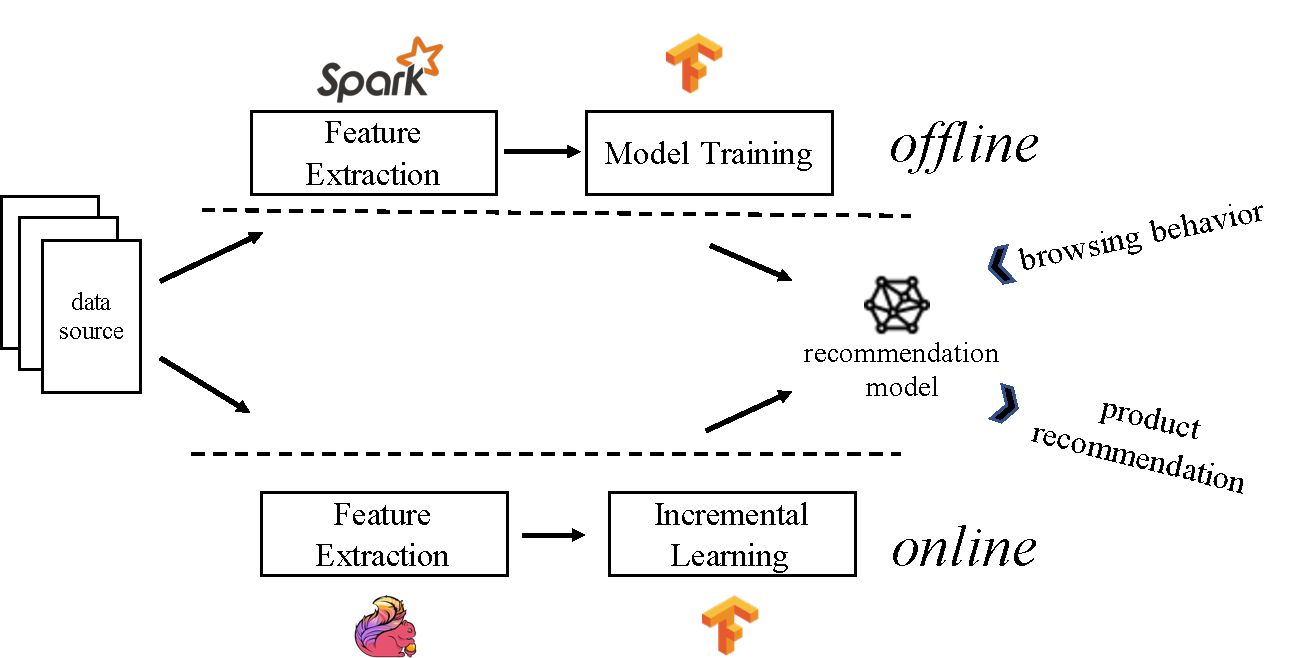
\includegraphics[width=0.8\linewidth]{figures/recommendation.pdf}
  \caption{Workflow of real-time recommendation}
  \label{fig:recommend-workflow}
\end{figure}
\fi

\begin{figure}
  \centering
  \subfigure[Word2Vec]{
  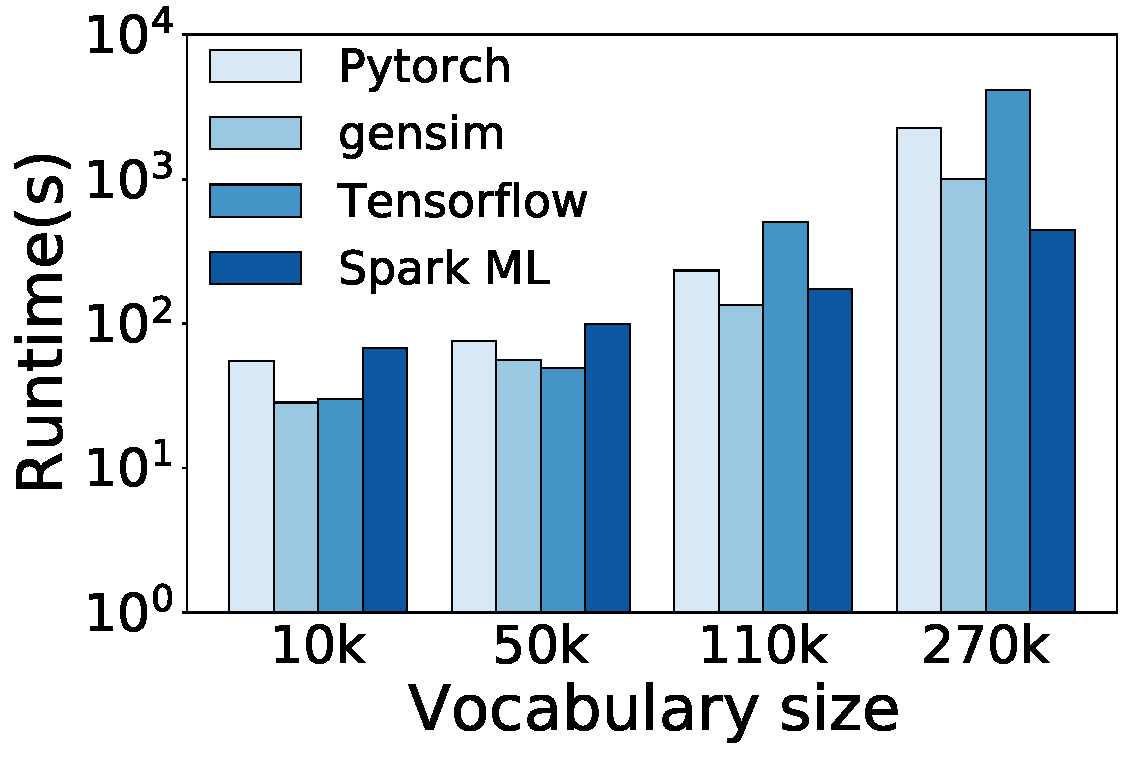
\includegraphics[width=0.45 \linewidth]{figures/chp2-word2vec.pdf}
  \label{fig:base-w2v}
  }
  \subfigure[PCA]{
  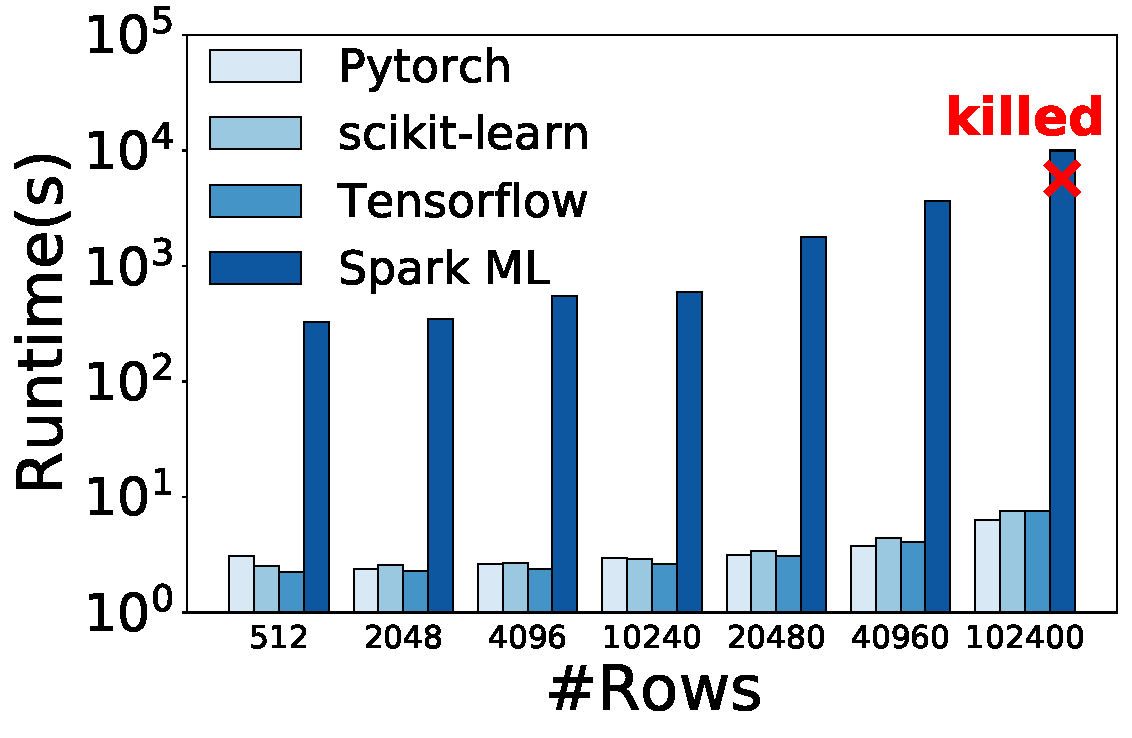
\includegraphics[width=0.45 \linewidth]{figures/chp2-PCA.pdf}
  \label{fig:base-pca}
  }
  
  \caption{Performance impact from different platforms}
  \label{fig:hetero}
%  \vspace{-20pt}
\end{figure}

\subsection{The State-of-the-Art Cross-Platform Data Analytics Frameworks}

Cross-platform computing can bring notable benefits, while building such a workflow first need to address several issues. Firstly, developers are required to learn the usages and programming models of the involved platforms, resulting in a high learning curve~\cite{gadepally2016bigdawg}. Secondly, to achieve the desired performance, developers need to choose appropriate platforms according to the workflow~\cite{agrawal2016rheem,hutchison2017laradb,gog2015musketeer}.
This gives rise to the study of the support for cross-platform computing, where a number of cross-platform frameworks are developed~\cite{tsoumakos2013case, tan2017enabling, lu2019multi,gittens2018accelerating}.
These works aim at addressing different issues, and we classify the state-of-the-art approaches into two categories.

\textbf{A unified execution engine} A class of work, e.g., BigDL~\cite{dai2019bigdl}, Spark~\cite{zaharia2016apache}, Ray~\cite{moritz2018ray} and LaraDB~\cite{kunft2019intermediate}, develops a big ecosystem and an universe API for performing tasks of a variety of domains. For instance, Spark’s execution engine supports not only map-reduce-style computing but also graph computing, machine learning, and SQL queries. This approach reduces programming efforts and mitigates the communication and data transfer overhead between tasks that were supposed to be deployed on two different platforms. However, it suffers from side effects of "one size fits all”. For example, Spark achieves suboptimal performance for specific tasks due to the different requirements for underlying storage and computing engines~\cite{anderson2017bridging, gittens2016matrix, gittens2018accelerating, dai2019bigdl}, such as the PCA algorithm shown in Figure \ref{fig:base-pca}. %Another issue is that it is hard to utilize existing platforms due to different programming languages or underlying architectures, demanding nontrivial development efforts.

\textbf{A framework that integrates existing platforms}    Another approach is to build a cross-platform framework that federates existing data processing platforms and provides a common interface to facilitate building cross-platform workflows~\cite{gog2015musketeer, agrawal2016rheem, hausenblas2013apache, beam2017apache, wang2017myria, dziedzic2016data}. Representative works include Rheem~\cite{agrawal2016rheem} and Musketeer~\cite{gog2015musketeer}. 
These frameworks provide an abstraction for building workflows. For cross-platform computing, a cost model is typically used to estimate the running time of each operator and select platforms that can improve the performance of a workflow. 
Specifically, Rheem uses a Java-based driver to drive workflow execution where tasks can only be executed on platforms with Java interface. This design excludes lots of well-known platforms such as PyTorch and Tensorflow. Differently, Musketeer translates front-end descriptions to common intermediate representations and then generates codes for selected platforms. In the paper, only SQL-like queries and vertex-centric graph are its supported front-ends, requiring significant development efforts to support complex data science workflows.

Previous works have enhanced cross-platform computing in multiple aspects and helped build efficient data science applications. Between the two types of approaches, the cross-platform framework is able to utilize existing data processing platforms which feature mature communities and well-tuned performance. We believe this is a promising direction for applying cross-platform computing to data science. 


\subsection{Deploying Data Analysis Workflows on the Cloud}

Cloud infrastructure provides virtualization technologies that encapsulate programs, dependencies and system settings in containers, where an instance can run with flexible resources and independent environments~\cite{wang2017myria}.
Therefore, cloud is a good candidate to meet the requirements in building cross-platform data analysis workflows.
To enable data analytics on the cloud, however, there are still several requirements and challenges to meet for a competent system.

\textbf{The impact of GPUs on platform selection} 
System hardware configurations have a huge impact on the performance of data processing~\cite{mattson2019mlperf}.
Cloud providers generally offer different cloud instances with flexible hardware resources like the existence of GPU, memory size and network speed.
Therefore, workflows from different users run in a variety of virtual hardware configurations and cluster scale, which influences platform selections for workflow operators. 

Figure xxx shows the GPU


\textbf{The impact of Network on platform selection}
Figure xxx shows different network speed

Although previous approaches adopt models in platform selection, their models are trained under specific hardware and software settings and cluster scale.
Consequently, it is hard to adopt such approaches in the cloud environment which can easily fail with a changing environment.
Overall, all the factors lead to the requirement for an efficient and robust hardware-aware platform selection algorithm for the cloud.


\textbf{Agile platform integration} Because data analytics workloads exhibit huge variance, there are a large amount of data processing platforms designed for specific workloads, and new data processing platforms are constantly emerging. 
To meeting users' demands and benefits the performance advantage from the new platforms, cross-platform frameworks need to adapt to the changes, which makes agile platform integration an essential feature. 
However, previous frameworks are designed with a tightly coupled architecture in which tasks of a workflow are executed by one driver program~\cite{balalaie2015migrating}. Consequently, integrating a new platform is expensive, which needs to rebuild, test, and deploy the entire project every time. 

Moreover, the model also need to be retrained which is time consuming. ++ intro to Rheem ML model.




%\textbf{Flexible Scaling} With tasks like data cleaning, filtering, and feature extraction, the input data for tasks in a workflow can be of huge variance. Therefore, a workflow demands different amounts of computational resources in its lifetime, which needs to be dynamically allocated at runtime. Moreover, flexibly scheduling tasks on specific nodes can help enhance the hardware utilization [osdi20xiao]. The architecture of current cross-platform frameworks tightly couple the development and deployment of platforms with the framework itself, and they typically initialize resources, like nodes in a cluster, before the workflow execution and occupy the resources throughout a workflow's life time. As a result, tasks of a workflow have to be executed as one instance, which leads to the same execution environment and hardware resources for all tasks. This design cannot adapt to changing workloads, resulting in either resource overprovisoning or low performance.

Considering all the potential issues in running cross-platform workflows on the cloud, it calls for a redesign of the architecture to adapt to the cloud environment for higher resource utilization.


\section{CLIC Overview}

\subsection{The Architecture of CLIC}

To address the above challenges in cross-platform computing, CLIC is designed as a cloud-native system with the major components running as multiple decoupled microservices and platform tasks running as separate jobs on the cloud.
CLIC formulates the platform selection as a classification problem and takes the input workflow as a graph, 
where Graphic Convolutional Network (GCN) is adopted for platform selection.
For the flexibility of expanding the fast growing platforms, the GCN model is made adaptive to new platforms without retraining the model.
Moreover, the model is designed as hardware-conscious to predict workflows with different computing resources.
All the aspects make CLIC a cloud native system that utilizes cloud environments to make it fault tolerant, flexible, scalable and adaptive.
Figure~\ref{fig:architecture} demonstrates the architecture of CLIC, which consists of three major components. 



\begin{figure}[tbh]
  \centering
  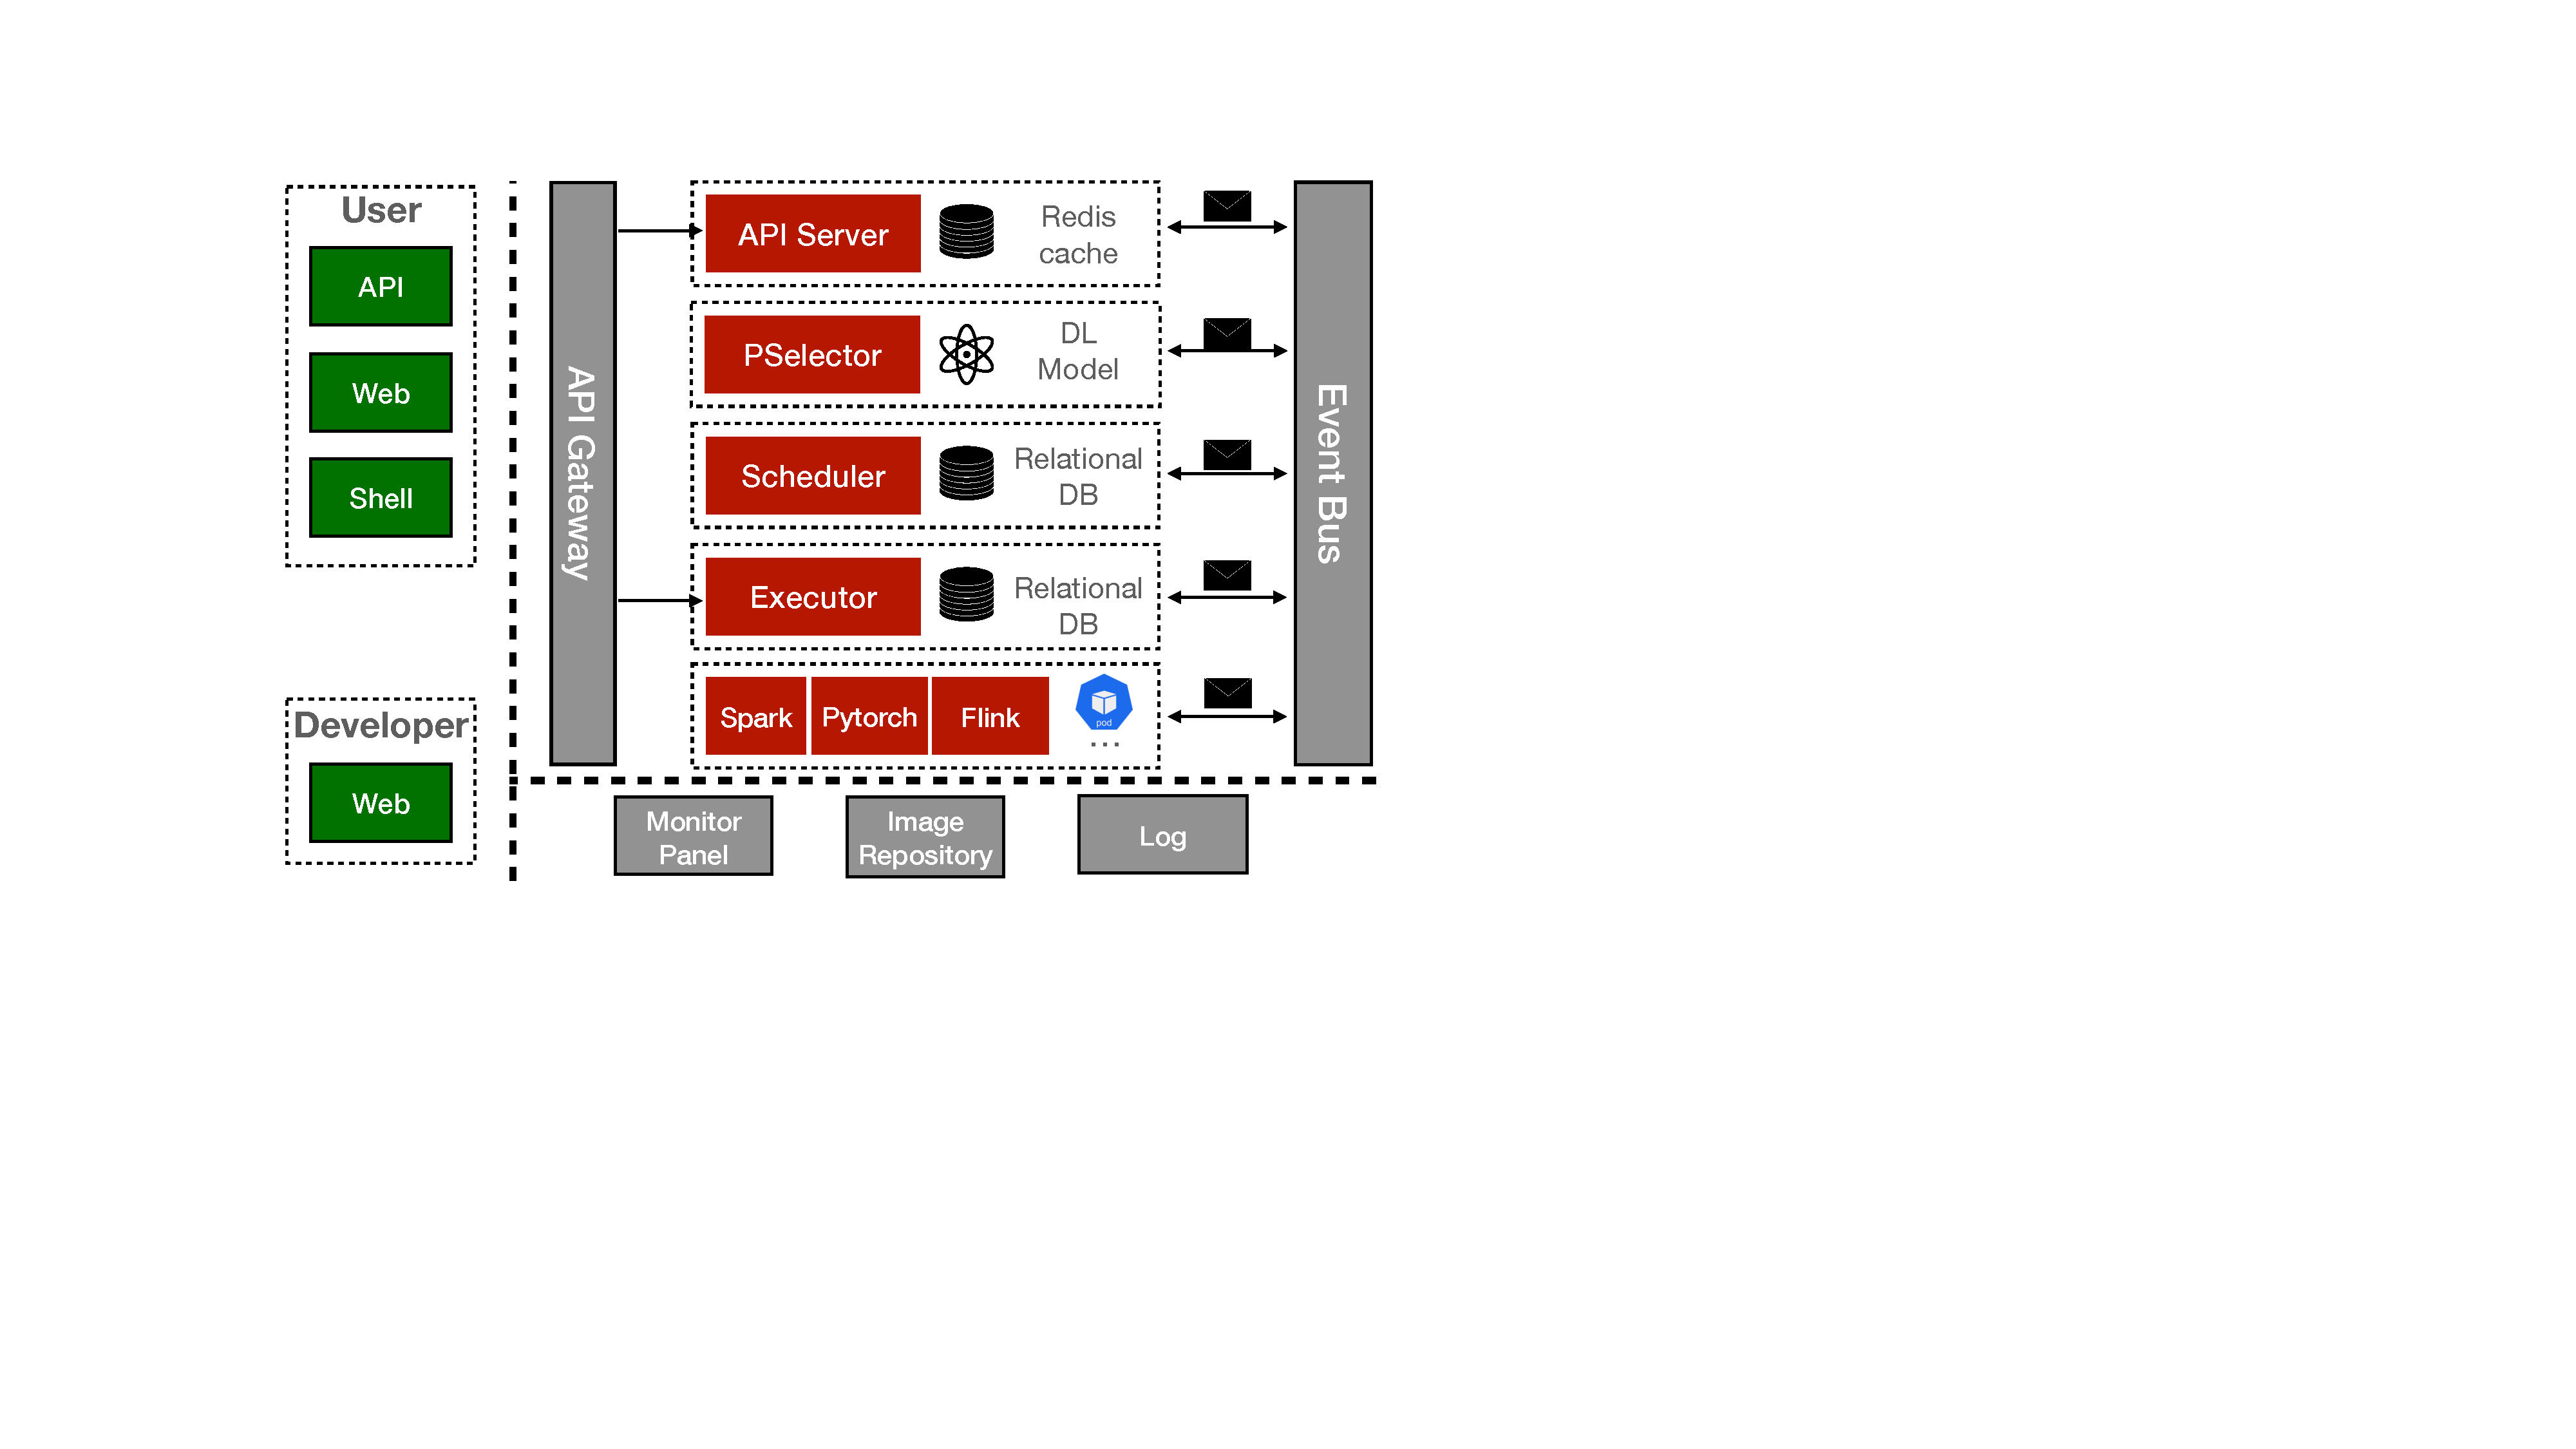
\includegraphics[width=0.8\linewidth]{figures/CLIC-arch-2.pdf}
  \caption{The architecture of CLIC}
  \label{fig:architecture}
\end{figure}

\textbf{Abstraction} CLIC provides a high level abstraction of a workflow, which uses platform-independent logical operators to express the computing tasks in it. 
A logical operator represents a basic computational task, such as data filtering or a K-Nearest-Neighbor(KNN) algorithm, which is platform-independent and only describe the computational semantics like functionality, parameter list, input/output data format.
The implementation of a logical operator on a speicific platform is called as a physical operator.
There is a 1-N (N $\ge$ 1) mapping between a logical operator and physical operators, which means a logical operator can be implemented on multiple data processing platform.
With a hardware-conscious GCN platform selection algorithm that optimizes overall workflow efficiency, each logical operator in a workflow is assigned with a data processing platform and becomes a physical operator.

Since platforms may have different data models, e.g., table, matrix/vector and graph, CLIC provides a set of data model transformation operators that developers can directly use to convert data models.
Besides that, a data model may have various data formats, such as a table can be row-based or column-based while the format a matrix can be block-partitioned or row-partitioned.
There exists no uniform data formats because the efficiency is dramatically diverse depending on computation patterns.
CLIC also provides a set of \textit{data source} and \textit{data sink} operators to deal with the data formats. A data sink operator serializes the data of a platform and write to file system with a specific data format, and a data source operator reads and deserializes data from files and converts to the desired formats for the following computing operators. Therefore, a data sink and a data source generally appear in pairs so that only one data format transformation is performed. 
By assigning operator platforms, merging adjacent nodes of the same platform as one job, and adding data source and data sink operators, CLIC reconstructs the logical workflow as a physical workflow for deployment.


 
\textbf{Service-Based Framework} To utilize the flexibility, failure recovery, and scalability of cloud, CLIC embraces microservices in the architecture, where each functional module is designed as a microservice, including API Gateway, Executor, Scheduler, and PSelector.
Microservices enable flexibility where each module can be devleoped, tested and deployed independently.
Specifically, domain specific functionalities such as the scheduling scheme can be developed with independent data storage, programming language and platforms, making the system highly flexible and extensible to integrate new schemes at runtime.
As shown in the figure, the CLIC server consists of a publish/subscribe mode event bus. All the microservices interact with each other by publishing and subscribing to a specific channel in the event bus.

The main microservices in CLIC are as follows. a) \textit{API Server} receives API calls from clients and responds to it whenver the result is ready. 
For example, when receiving a configuration lookup request, API Server publishs the event to the specific channel and starts to listen. 
After configuration microservice responds and API server receives the result ready event, it wraps the result with headers and responses to the client. 
In this microservice, in-memory key-value stores is used to cache query results to speed up the process.
b) \textit{PSelector} takes a logical plan as input and outputs a physical plan with each operator being assigned with a platform. Inside the PSelector, it utilizes a GNN model to predict platforms. 
We detailedly describe the approach in Section 4.  
c) \textit{Scheduler} records the status of all resources and specifies the number of container instances and the targeted nodes to be deployed etc.. 
The resource status are periodically retreived from Executor and maintained in the Scheduler's database. 
With the microservice architecture, different scheduling policies can be developed as independent microservices and deployed according to requirements of production systems.
d) \textit{Executor} controls the underlying container resources using the Kubernetes API and submits jobs for execution. The controlment includs instantiating, pausing, destroying the container and restarting jobs whenever it fails. All the platform-related configuration files like container and network are declared in the form of YAML and managed by Helm~\cite{} charts and passed to the deployed platforms in execution.
The four core components of CLIC are developed and deployed independently, making CLIC a flexible system with high availability.



\textbf{Cloud-Native Task Deployment} Besides designing the cloud-native framework, CLIC decouples data processing platforms from the framework to facilitate extensible platform integration and independent deployment.
All physical operators of a platform are built in an image, thus each platform is developed and maintained independently.
Moreover, one platform of different versions are kept as separate images to provide backward compatibility.

To mitigate expensive data transfer between operators, the input and output of an operator is an abstraction of the platform (e.g., RDD or numpy.array) or a specific data structure (int [] in C).
In this way, when adjacent tasks belong to the same platform, they can be merged and deployed as one job.
Instead, tasks of different platforms are launched as separate jobs and passes data through a file system.
After platform selection, each task in a workflow is assigned with an image of its corresponding platform.

To execute physical operators in one job, a platform image contains a driver program to drive the workflow execution. 
In the deployment of a job, Executor passes the operators information of the job to the driver program in the platform image. 
The driver program calls the specified data source operator to read data from the file system and transfers into the input abstraction and formats of operators, such as building an RDD. Then driver program interprets the workflow, calls the corresponding operators and passes data one by one. In the end, the driver program calls the data sink operator to serialize data and write to specified directory in the file system.
Overall, CLIC merges and deploys operators of the same platform as one task while automatically connecting adjacent platforms with automatic data transformation. 





\iffalse
\textbf{Platform-agnostic Programming}   We thin wrap each integrated platform's API to offer a logical operator set and provide various data models like the vector/matrix in linear algebra. The logical operator describes only the computation semantics like functionality, parameter list, etc.. User can build platform-agnostic workflow using the logical operator set and data models, and run it on any (integrated) platform. This greatly alleviates users burden of struggling in the overwhelming platforms.

\textbf{Cross-platform Computing}        To support building the cross-platform workflow, we (i)offer corresponding logical operator sets and data models for different computing paradigms, and (ii)implement a series of data model conversion and data transmission operators to bridge operators from two paradigm. For example, to support both relational and linear algebra we first provide relational operators along with its table model as well as linear operators along with its vector/matrix models, and then implement a conversion operator that assigns each column a name(column number) and a data type to transform a matirx to table.

\textbf{Automatic Platform Selecting}    CLIC can automatically convert the logical plan to the physical plan, i.e. select a platform for each logical operator. To achieve this, we introduce an end-to-end GNN-based model that takes as input a logical plan and outputs the platform-specific physical plan that has the lowest cost. Each logical operator in the logical plan is vectorized using our novel feature extraction method.

\textbf{High Availability}               The high availability is ensured by (i) status monitor, (ii) container self-healing mechanism and (iii) data recovery. With the help of ZooKeeper, we implement health check and progress reportor to monitor the status of the running jobs. When the job fails, CLIC will instantiate a new container and restart the job using Kubernetes self-healing mechanism. The input data is recorverd from checkpoints that are implicitly inserted (by the Planbuilder ?).

\textbf{Agile Integration}               We containerized each platform along with its neccessary components like the above progress reportor, so that dependency management and environment setup should be a lot easier. What's more, we apply semantic versioning on the integrated platforms to avoid conflicts like expired API call after iterate updates. Apart from that, thanks to the feature extraction method, the GNN-model doesn't need to be retrained whenver there's a newly operator/platform anymore, i.e. is compatible for an integration.

%\subsection{CLIC Architecture} 
Figure \ref{fig:architecture} demonstrates the architecture of CLIC that consists of the clients(left), the CLIC server(right top), and 3rd-party services.

\textbf{Client}  There're two types of clients for different roles: user and developer. The user programmes the workflow using clients like native lanuage API, Web interface or command line. The user client wraps the workflow with headers and sends to the CLIC API server for execution. The developer client is a developer toolkit for registering configuration, observe and manage the cluser, etc.

The CLIC server consists of a series of microservices and a publish/subscribe mode event bus. All the microservices interact with each other by publishing and subscribing to a specific channel in the event bus. The main microservices are as follows:

\textbf{API Server}  The API Server receives the API call from clients and respondes to it whenver the result is ready. For example, when receiving a configuration lookup request, it publishs the event to the specific channel and starts to listen. After receiving the result ready event, it wraps the result with headers and responses to the client. At last, we use redis database to cache some of the query result to speed up the process.

\textbf{PSelector}   PSelector takes a logical plan as input and outputs a physical plan whose operator is assigned a platform. Inside the PSelector, it utilizes the prementioned GNN model to determine the platform. Notice that, the GNN can also be replaced by other models like ML-based models or heuristic methods as long as their input format is aligned.

\textbf{Scheduler}   The Scheduler specifies the number of container instances, target nodes etc. given the current resource utilization. The resource status are periodically retreived from Executor and maintained in the Scheduler's database.

\textbf{Executor}    The Executor controls the underlying container resources using the Kubernetes API and submits the jobs to them. The controlment includs instantiating, pausing, destroying the container and restarting jobs whenever it fails. All the platform-related configuration files like container and network are declared in the form of YAML and managed by Helm charts.
\fi

% We propose CLIC, a highly extensible cloud-native framework for cross-platform computing. To address the above challenges, we decouple data processing platforms from the underlying framework to facilitate independent development and deployment.
% CLIC divides a workflow into multiple \textit{tasks} where adjacent tasks belong to different platforms and are launched as separate instances.
% To express cross-platform workflows, CLIC uses \textit{logical operators} as the abstraction, where each logical operator describes a minimal functional unit.
% A \textit{physical operator} is the implementation of a logical operator on a specific platform, thus there may exist a one-to-many mapping between a logical operator and multiple physical operators.
% With all physical operators of a platform being built as a container image, each task in a workflow is associated with an image of its corresponding platform. This design enables agile platform integration where new platforms can be developed and integrated in a plug-and-play mode, without rebuilding the entire framework. By maintaining platforms with diverse versions and system configurations with images, CLIC provides backward platform compatibility and consistent performance. 
% The architecture of CLIC helps maintain independent development and deployment environments.

%To enable dynamic scaling in a workflow, we implement a scheduler to specify needed resources for each task at runtime.




\iffalse
Figure \ref{fig:architecture} demonstrates the architecture of CLIC, which consists of four major microservices, i.e., PlanBuilder, Optimizer, PSelector, and Scheduler. PlanBuilder provides the information of logical operators to build the \textit{logical plan} of a workflow (step 1). The logical plan is sent to Optimizer for potential optimizations, and then sent to PSelector to assign platforms by mapping \textit{logical operators} to \textit{physical operators} with a GCN model (step 2). The output of PSelector is the \textit{physical plan}, which is used by Scheduler to deploy corresponding tasks on the cloud. 
When the physical plan of a workflow arrives, Scheduler launches instances of the selected platforms subsequently and scales them according to workloads (step 4). An instance of a platform contains an Executor that receives and translates the physical plan from Scheduler and calls the specified physical operators. Deploying a workflow with multiple tasks requires monitoring their running states of tasks. As shown in the figure, Executor regularly sends heart-beats with its running states to Scheduler. It is worth noting that, to support QoS requirements of various workflows, Scheduler provides interfaces to develop different resource allocation schemes for flexible scaling.
\fi

\iffalse
In CLIC, adjacent operators that run on the same platform are deployed as one Kubernetes task. We store physical operators developed on a platform (a specific version) as a container image. It contains all physical operator implementations and an Executor that translates the physical plan and executes the corresponding operators. Developers can build their own images after adding or re-implementing new operators on a platform. After updating the image information and corresponding operator mappings in the configuration server, developers can run workflows with their newly developed platforms and operators without affecting other workflows. In this way, CLIC enables flexibility in both development and deployment, which fits for the requirements of data science applications.

CLIC is a cloud-native computing framework designed for cross-platform data science workflows. CLIC integrates platforms from various domains and provides a consistent programming model, including multiple data models and algebras. CLIC selects platforms for a given workflow using GCN to optimize the overall performance. What’s more, CLIC enables passing UDF and dynamic control flow for building advanced workflow. Last but not the least, CLIC encapsulates components as containerized \textit{Microservices} and deploy them on the Kubernetes.

In order to integrate multiple platforms and offer a unified programming model, CLIC decouples the operator’s semantic and execution to the logical operator and the physical operator. The logical operator is used for declaring a workflow. It only describes the properties like the parameter list, return value, etc. and is not associated with any platform; The physical operator is the corresponding executable implementation on a specific platform. The mapping relationship between the logical and physical operator is 1-n. Programmers can construct the workflow using only logical operators without knowing the underlying platforms and CLIC can improve workflow performance by selecting the best physical operators.

The PlanBuilder offers data scientists multiple data models and logical operators to build the workflow. The provided data models including table, vector, matrix and graph, and the provided logical operators including various algebraic operations, data model conversion algorithms, and control flow primitives. The Planbuilder organizes the workflow as a DAG form logical plan composed of logical operators and their dependencies (step 1). The logical plan is then sent to the Middleware.

The Middleware contains a SQL parser, several optimization rules, and the GCN, which optimize the logical plan and determine physical operators (step 2). It returns the optimized logical plan to the PlanBuilder. After that, the adjacent logical operators bound to the same platform are grouped as sub-logical-plans and sent to the Scheduler (step 3). 

Scheduler is responsible for multi-task scheduling. It manages all workflows’ running states in the configuration server, as well as other meta information such as platform configurations, logical/physical operator properties, the operator mapping table, etc. When a new logical plan arrives, the Scheduler starts a specific number of instances of the determined platform based on workloads and sends the logical plan (step 4). 
\fi


% \begin{figure*}
%     \centering
%     \subfigure[Original logical plan]{
%         \label{fig:dag1}
%         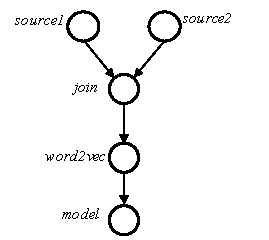
\includegraphics[width=0.18\textwidth]{figures/dag1.pdf}
%     } 
%     \subfigure[Optimized logical plan]{
%     \label{fig:dag2}
%         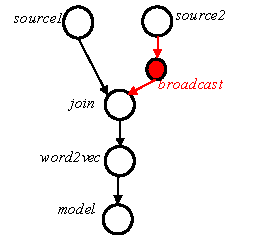
\includegraphics[width=0.18\textwidth]{figures/dag2.pdf}
%     } 
%     \subfigure[Platform selection]{
%     \label{fig:dag3}
%         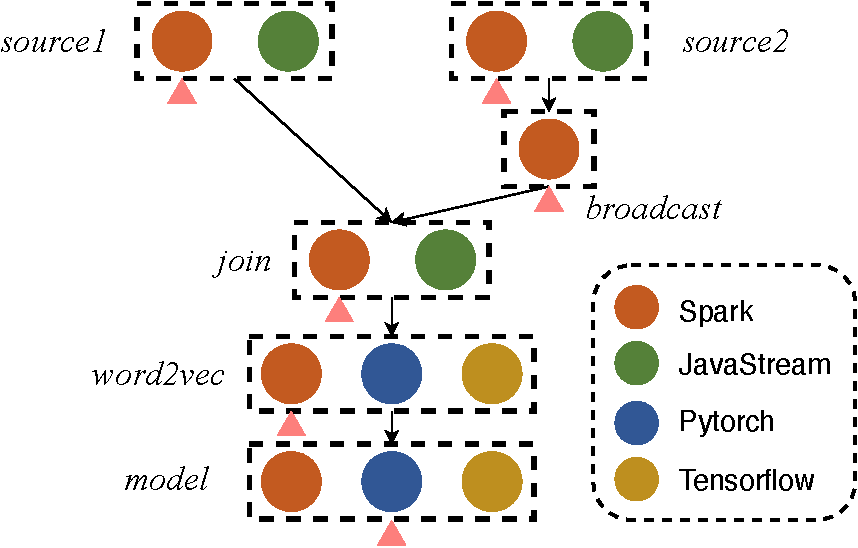
\includegraphics[width=0.27\textwidth]{figures/dag3.pdf}
%     }
%     \subfigure[Physical plan]{
%     \label{fig:dag4}
%         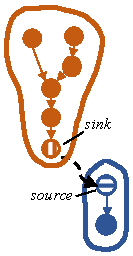
\includegraphics[width=0.1\textwidth]{figures/dag4.pdf}
%     }
%     \vspace{-5pt}
%     \caption{The case of running sentiment classification in CLIC}
%     \label{fig:optimizing-process}
%     \vspace{-5pt}
% \end{figure*}


\subsection{Case Study}
We adopt sentiment classification as a case to demonstrate how CLIC works. It is a common nature language processing task that classifies documents based on the semantics. The data processing tasks mainly include data ETL (Extract, Transforming, Loading) and training of a classification model. The pseudo-code of a simple implementation is shown in Listing \ref{code:workflow}.

\begin{listing}[ht]
\begin{minted}[frame=lines,
framesep=2mm,
baselinestretch=1.2,
fontsize=\footnotesize,
linenos]{python}
source1 = read('BBC-News.txt’)
source2 = read('Hamlet.txt')
corpus = join(clean_source1, clean_source2)

word_embedding = toMatrix(clean_corpus, Word2Vec)
    
model = Model('LSTM')
train(model, word_embedding['train'])
topic = test(model, word_embedding['test'])
\end{minted}
\caption{Pseudo-code of sentiment classification in CLIC}
\label{code:workflow}
\end{listing}
The processing steps are as follows. 1) Based on logical operators, PlanBuilder builds the logical plan for the workflow. As shown in Figure \ref{fig:dag1}, the logical plan is a  DAG consists of five logical operators. 2) Optimizer applies optimizations on the logical plan. In this case, because the data volume of \textit{source2} is way lesser than source1, CLIC implicitly inserts a \textit{broadcast} operator to put \textit{source2}’s data on all nodes in order to reduce communication times. The optimized logical plan is shown in Figure \ref{fig:dag2}. 3) Logical operators are assigned to platforms with a GCN model. Figure \ref{fig:dag3} shows the potential platforms of each logical operator and marks the selected platforms with red triangles. Two platforms are selected in this case, where model training is placed on Pytorch while the rest operators are assigned to Spark. 4) The adjacent Spark operators and the PyTorch operator are grouped into two tasks as shown in Figure \ref{fig:dag4}, because merging adjacent operators of the same platform as one task can mitigate data transfer overheads. Then Scheduler chooses the corresponding container images for the two tasks and deploys them on the cloud subsequently. Note that, in the generation of the physical plan, PlanBuilder implicitly inserts a \textit{sink} operator in Spark to output the intermediate results and a \textit{source} operator in Pytorch to read Spark’s results.

\section{SYSTEM DESIGN AND IMPLEMENTATION}
In this section, we describe the design and implementation of CLIC, including the support for agile platform integration, environment management, and the supports for developing cross-platform work- flows. 
The prototype of CLIC is built on Kubernetes, with the mod- ules and tasks running in Docker containers.

\subsection{Operator Mapping and Management}
CLIC provides a logical operator set that is a union of operators from multiple domains. 
For instance, the batch processing operator subset consists of MAP, FLATMAP, SORT, FILTER, etc., 
and the linear algebra subset consists of DOT PRODUCT, MULTIPLY, TRANSPOSE, and so on. 
A logical operator describes the operator name, input parameters, return value, algebra type, and related optimizing information. 
The information of all operators is stored in a configuration server and provided to developers by PlanBuilder. 
A physical operator contains information including the name of the physical function and data types on the platform. 
Each logical operator needs to be mapped to a physical operator for execution, i.e., assigning a platform to an operator.

\begin{center}
    \begin{tabular}{ c c c }
        Logical Operator & Platform & Physical Operator \\
        \multirow{3}{2em}{PCA} & Tensorflow & pca() \\
        %  & PyTorch & low_rank() \\
        %  & Spark ML & PCA() \\
        \multirow{2}{4em}{Map} & Spark & map() \\
         & JavaStream  & map() \\
        \multirow{3}{4em}{Word2Vec} & PyTorch & Word2Vec() \\
         & Spark ML & Word2Vev() \\
         & Gensim & Word2Vec() \\
    \end{tabular}
\end{center}

According to the workflow and workload, different physical operators can be chosen for deployment. 
We maintain an operator mapping table that contains one-to-many mappings between logical operators and physical operators. 
Table 1 exemplifies the mappings of three logical operators, i.e., PCA, Map, and Word2Vec. 
As listed in the table, Map has the implementation on Spark and JavaStream, while PCA and Word2Vec can be mapped to machine learning platforms including PyTorch and Tensorflow. 
When a logical operator does not have an equivalent native implementation on a platform, developers can implement it and update the mapping table, such as the customized Word2Vec operator in PyTorch. 
In the configuration server, the operator mapping table is maintained with the support for insert, delete, and replace operations.

\subsection{Image Management}
CLIC facilitates the integration of new platforms by maintaining them as images. 
The metadata of each image is stored in the image table on the configuration server, including Dockerfile, platform version, entry-point, and all available physical operators. 
In the image table, images of the same platform are stored together, and each image contains the platform of a different version. 
With the physical plan of a workflow being split into tasks on different platforms, a proper image is located and used for each task. 
When there exists different versions of the same image, the latest version that contains the required physical operators is selected.

To integrate a new platform, the image needs to be built with the corresponding information being updated in the image table.
If a new operator of a platform is developed, besides rebuilding the image and updating its information in the image table, 
the information of the new operator also needs to be updated in the operator mapping table.


\subsection{Supports for Building Cross-Platform Workflows}
Building a cross-platform data science workflow demands a set of functionalities and supports. 
In this section, we introduce the data model conversion, UDF passing and dynamic control flows in CLIC.


\textbf{Data Model Conversion} 
There can be significant differences between data models of different platforms.
For example, an array’s dimensions implicitly order cells while is different from a Table (SQL tuples) [34]; 
The graph model can perform better on relationship queries than the Table due to the inherent structural differences [27, 31]. 
These differences make it hard to construct a unified data model that can be used by all operators. 
Therefore, we bridge the gaps between data models by implementing a series of model conversion algorithms. 
The toMatrix operator in line 5 of Listing 1 is one of the conversion algorithms that converts a concrete word to a dense vector using the skip-gram [29] algorithm. 
Note that we provide essential conversion algorithms in our model conversion library, such as the skip-gram, and expose interfaces to develop conversions concerning business logic.

\textbf{UDF}  Due to the decoupled architecture, a user-defined function (UDF) is passed to a platform driver through RPCs. 
In CLIC, a UDF instance is firstly serialized and embedded in the logical plan by the Planbuilder. 
It is deserialized by the Executor inside the underlying platform to drive the execution. 
One tricky problem is when the UDF is implemented in a different lanugage with the underlying platform. 
CLIC currently supports translating UDFs between Python and Java using a 3rd-party tool.

\textbf{Dynamic Control Flow} We introduce control flow operators including SWITCH, NEXT ITERATION, and EXIT to help build workflows with iterations. 
The SWITCH primitive takes an if-statement as the input parameter, initial iteration flag values as input data, and returns a boolean value that directs the executor. 
The NEXT ITERATION operator takes iteration flags as input data and forwards them to the head of the next iteration block, e.g. SWITCH operator. 
EXIT operator indicates the end of an iteration and connects to the next operator in the workflow.
A simple workflow with iteration is shown in Figure 5 where $i$ is the iteration flag, $i < 10$ is the if-statement, and Map operator is the iteration body.

\subsection{Optimizing Logical Plan}
Optimizing the logical plan of a workflow can bring notable performance improvement [17, 22].
In CLIC, we implement optimizers as microservices, and two currently supported optimizers are illustrated as follows.

\textbf{Align Layout}
Access patterns (row-, column-, or block-wise) of linear algebra operators can significantly impact ML workflow performance [39]. 
For example, the matrix multiplication operator access the left matrix in a row-wise pattern and access the right matrix in a column-wise pattern. 
Changing the sparse matrix layout to match the access pattern can significantly improve the performance [25]. 
CLIC identifies the pattern of the sparse matrix multiplication and implicitly inserts a layout conversion operator.

\textbf{Broadcast}
Some binary operations like JOIN and MATRIX MULTIPLY need to frequently send data batches between nodes when input data is distributed stored. 
However, when one of the data is small enough to fit in memory, such as multiplying a matrix with a vector or joining a big table with a tiny one, the coordinating overheads can be eschewed by broadcasting the small one to all nodes so that they can be computed locally [8, 26].
CLIC identifies this pattern and implicitly inserts the BROADCAST operator.



\section{Selecting Platforms in CLIC}
The platform selection is to find the platform with the lowest cost for each logical operator in the logical plan. We take this problem as a node classification problem, where the platform of the lowest cost is considered as the label of the logical operator. We use the GCN as the classifier, which is considered more suitable for node classification problems. Below we first narrate the feature extraction method used in CLIC and then describe the classification method using GCN.

\subsection{From One-hot Encoding To Embedding}
The traditional one-hot encoding method used in [rheem, ml-based] to treats each operator as a dimension to vectorize the operator as a 0-1 vector. 
Its dimension equals to the number of operators and each vector only has one non-zero value, therefore the one-hot encoding is always high-dimensional and sparse. 
Generally speaking, this methoid is less computational since the majority of neural network toolkits do not play well with very high-dimensional, sparse vectors [Neural Network Methods in Natural Language Processing, 2017].

Besides, the one-hot encoding is imcompatible to a new operator which goes against our high extensible character. 
In particular, the one-hot encoding needs to increase the dimension of all operator vectors whenver a new one is inserted. 
Figure xx examplified this situation where as the new Flatmap operator (red one) being inserted, all the vectors' dimension are grown. 
Thus the previous model needs to be retrained otherwise the new vector becomes an invalid input due to its higher dimension. 
Even if reserving some empty dimension to stablize the input, the model still cannot properly classify the new operator because the new dimension is orthogonal to the other dimension and the model lacks knowledge about this new dimensions.

In order to overcome the above two problems, we turned our attention to using the embedding to represent the operator. 
In mathmatic, an embedding is a function f X -> Y that maps a data point X in one space to point Y in another space. 
This is the most important preprocess technique in natural language processing (NLP), where the word embedding is a term used for the representation of words for text analysis. 
It is typically in the form of a real-valued vector that encodes the meaning of the word such that the words that are closer in the vector space are expected to be similar in meaning [wiki]. 
For promotion, there also are image embedding, video embedding, and of course, operator embedding. 

The Operator embedding is a representation of an operators in the Euclian space. 
We can share the same idea in the word embedding that allows semantically similar operators to have closer distance. 
Figure xx outlines the embedding structure. 
It can be seen that (i) the dimension of the vector space is independent of the number of data points and is usually much smaller than that of the one-hot encoding []. 
In short, the embedding is dense and low-dimensional, therfore more computational; 
(ii) the embedding of the old and new operators are in the same Euclidean space and the embedding includes the semantic relationship of the operators, 
therefore the model can make inference directly for the new operators using the existing knowledge. 

\begin{figure}
    \subfigure[One-Hot Encoding]{
        \label{fig:one-hot}
        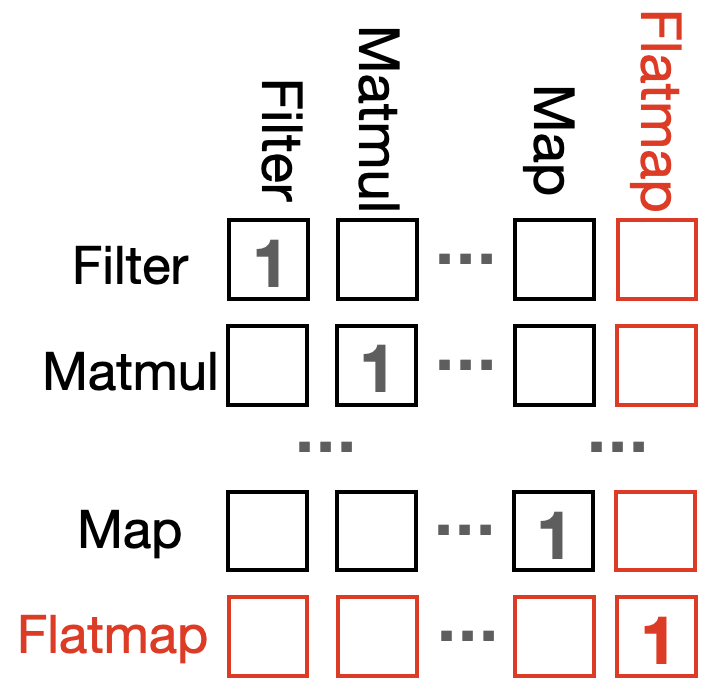
\includegraphics[width=0.3\linewidth]{figures/one-hot.png}
    } 
    \subfigure[Operator Embedding]{
        \label{fig:embedding}
        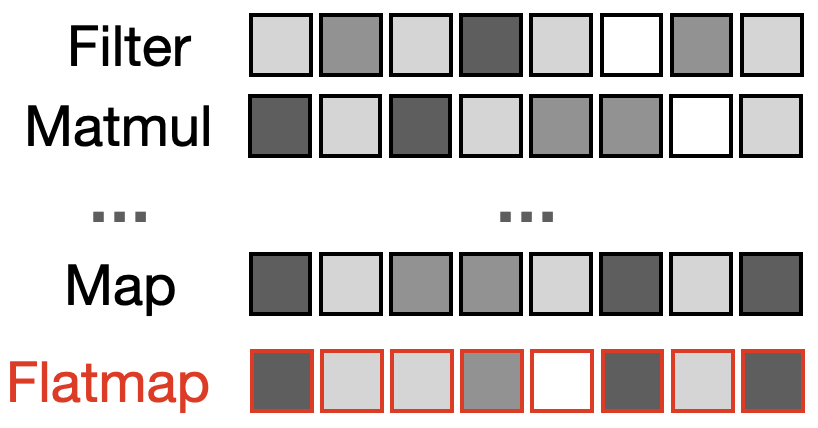
\includegraphics[width=0.3\linewidth]{figures/embedding.png}
    } 
    \caption{Vectoization Method}
    \label{fig:encoding}
\end{figure}


\subsection{GCN Intuition}
Graph Convolutional Network is a convolutional neural network that can be directly applied to graphs. 
It stacks layers of learned first- order spectral filters, which are followed by an activation function to learn graph representations [42].

‘Convolution’ in GCN refers to multiplying the input matrix with a set of weights that are commonly known as filters or kernels. 
The filters act as a sliding window across the matrix and enable GCN to learn features from neighboring cells. 
Before convolution, there needs a extra normalization step to change the irregular topology into matrix. 
Figure XX shows the node classification process of one operator using GCN. 
It first traverses each operator in the logical plan and samples K (a hyperparameter) neighboring operators to form a K*|V| matrix where E indicating the length of operator's feature vector. 
If the operator has less than K first-level neighbors, then it adds second-level neighbors. 
Then it applys the kernel across the matrix and gets the vector that contains the topological information. 
After that, the vector is fed into the neural network to compute its graph representation that can be used to classify. 
Finally, we use the MLE as the loss function to compare the graph representation and the platform embeddings and update the GCN.


\begin{figure}
  \centering
  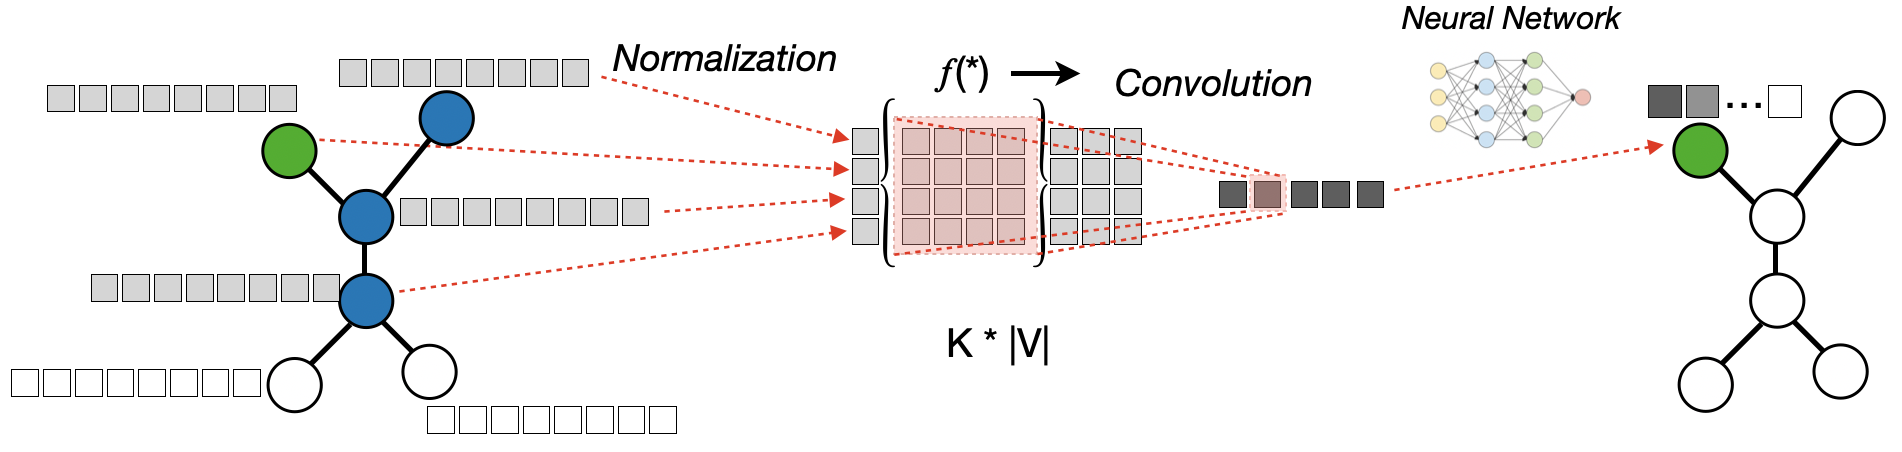
\includegraphics[width=\linewidth]{figures/gcn.png}
  \caption{Selecting platforms with GCN}
  \label{fig:gcn}
\end{figure}

\subsection{Data Generation}
\textbf{Generating Operator Embedding}
In word embedding, because the words in a sentence have certain correlation with its context words, 
therefore the cost function of training Word Embedding is to maximum the joint probability of the word and its context words. 
Similarly, we can also reasonably assume that the operators that appear in a same logical plan have more association and use the same cost function. 
We take the topological-ordered logical plan as the sentence and the logical operators inside are words, 
then use the same model to train the operator embedding. The results are shown in Figure xx. 
For the sake of visualization, we just show the top-2 dimensions with the highest eigenvalue. 
One observation is that operators that are the same computing paradigm and have the same number of inputs and outputs tend to have small cosine distance. 
What's more, the newly inserted Flatmap operator is also mapped closer to the Map operator instead of the Matmul operator which is probably due to the same reason.

It's important to emphasize that the operator embedding technique is not bound with CLIC but a general feature extraction method. 
One can generate an operator embedding whether the operator is supported by CLIC or not as long as there are logical plans that contain this operator.

As we have mentioned that the operator embedding is compatible for the newly integrated operator. 
There're two cases when integrating a new operator:
\begin{itemize}
    \item [1)]
    The operator is new to CLIC but not the model, therefore its embedding can be retreived in CLIC directly from the model.
    \item [2)]
    The operator is also new to the model, i.e. the "OOV" (out of vocabulary) problem. 
    In this case, the model needs some new training data to recognize it. 
    Therefore, we synthesize some new logical plan that contains the operator according to operator's attributes and then incrementally updates the model to generate the embedding.
\end{itemize}

Apart from the above operator embedding, 
we also design and generate the embedding for each physical computing platform. 
The mathmatical meaning and generation method goes the same. 
We don't further explain due to limits of space.


\textbf{Generating Training Data}
The effectiveness of the GCN strongly depends on the training data. 
In our case, a large amount of disparate logical plans (data points) together with the best physical platform (labels) of each logical operator in it is required. 
The logical operator's feature vector is composed of two parts: operator embedding and the global hardware resources. 
The latter is the same for the operators in the same logical plan, including infrastructure's CPU frequency, main memory, GPU memory, network bandwidth, etc. 
However, there is currently a lack of the Workflow dataset for cross-platform computation, so we borrow the TDGen [] to synthesized datasets separately for each computation mode and on different infrastructures.

\section{Experiment}
We design and perform several experiments to evaluate our framework and prove that CLIC is capable of 1) selecting a suitable platform based on the workload and 2) building and running workflows on multiple platforms that are not supported by existing frameworks. 

\subsection{Experimental Setup}
All experiments are conducted on a cluster of 3 nodes, where each node is equipped with two 2.3 GHz Intel Xeon Gold 5218 processors with 16 cores, four 32GB DDR4 RAM, 2TB SSD and runs on 64-bit Ubuntu 20.0.1. The platforms deployed on the cluster include Java’s Stream library (JavaStream), Spark 2.4.5 (Spark), Spark ML 2.4.5 (Spark ML), GraphX 2.4.5 (GraphX), JgraphT 1.4.0 (JgraphT), GraphChi 0.2.2 (GraphChi), Giraph 1.3.9 (Giraph), PyTorch 1.7.1 (PyTorch), python gensim library (gensim). The platform images and containers are managed by Kubernetes v1.20. Alluxio 2.4 is used for data orchestration and HDFS 3.2.1 works as the backend file system.


\subsection{Performance Evaluation of A Single Operator}
\begin{figure}
  \centering
  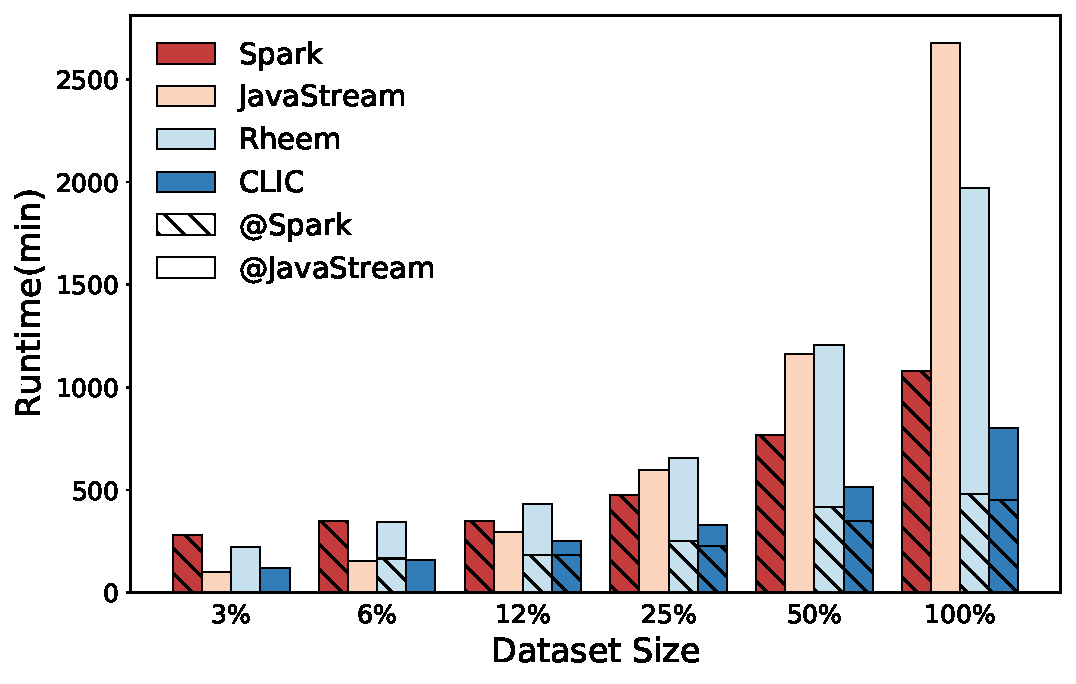
\includegraphics[width=0.7\linewidth]{figures/chp6-CrimeStage.pdf}
  \caption{Performance of London crime analysis}
  \label{fig:exp-crime}
\end{figure}

Figure \ref{fig:single-opt-selection} shows the performance of four representative operators i.e., Word2Vec, PCA, PageRank, and WordCount. In the figures, the platform chosen by the GCN model in CLIC is indicated by red stars. In the evaluation of Word2Vec (Figure \ref{fig:single-word2vec}), we use the NLTK dataset containing the different sizes of corpora to represent different workloads. Among supported platforms, gensim achieves the highest performance when using the corpus of 10k vocabularies while Spark ML suffers from the distributed communication overheads. However, Spark ML gains a performance advantage when the corpus contains 270k vocabularies. This is because Spark ML is able to utilize multiple nodes for the enlarged dataset, where the communication overheads become subtle compared with the computing time. CLIC identifies the difference and selects the best platform in both situations. Figure \ref{fig:single-PCA} shows the accumulated time of 10 PCA runs. The dataset is the Hotel Booking Demand \footnote{https://www.kaggle.com/jessemostipak/hotel-booking-demand}. Consider that running PCA in a single time has negligible performance difference on PyTorch, scikit-learn and Tensorflow for all dataset sizes, we set the feature vectors of these physical operators as the same to reduce the data amount required by training the GCN. Therefore, CLIC selects PyTorch all the time. The data set in evaluating PageRank is the Twitter follower network\footnote{https://snap.stanford.edu/data/twitter-2010.html}. As shown in Figure \ref{fig:single-PR}, JgraphT achieves the highest performance when the graph contains less than 1.8 million vertexes while Giraph performs the best on the other cases for its higher efficiency in processing large graphs. To evaluate the map-reduce operators, we encapsulate the WordCount as a coarse-grained operator. As shown in Figure \ref{fig:single-wc}, the single-machine framework JavaStream achieves the highest when the corpus is small. Instead, Spark is 4.2X faster than JavaStream when using the full dataset because it can be divided and computed locally on each node with little global synchronizing overheads. CLIC selects the best platform for both the PageRank and WordCount operators.

The above experiments validate that CLIC is capable of enhancing the performance of an operator by selecting its appropriate platform.

\subsection{Performance Evaluation of A Big Data Workflow}

Figure \ref{fig:exp-crime} compares the performance of a workflow that analyzes the London Crime dataset\footnote{https://www.kaggle.com/LondonDataStore/london-crime}, which size is 28 GB. The dataset describes the amounts of criminal reports by month, major/minor category, etc. We use percentages in the figure to denote different sizes of the dataset. For instance, 50\% means the execution time on only 14 GB of data (28$\times$0.5).

The workflow mainly consists of the following four procedures: 1) reading data and transforming it to a computable format; 2) filtering reports to preserve only the ones with certain crime types, which will remove 90\% of the data; 3) sorting and transforming reports to a human-readable format, and 4) grouping reports based on quarter. We evaluate the performance on JavaStream and Spark, as well as cross-platform frameworks Rheem and CLIC. 

The observation is that when the data size is less than 6\%, the computational efficiency of native Java and CLIC is 2.1$\times$ higher than Rheem and 2.8$\times$ higher than Spark. The reason is that Spark is always set to use all available nodes in a cluster even when the dataset is small. Consequently, the communication overheads among distributed workers dominate the execution time. Both CLIC and Rheem select the JavaStream for all operators in a small dataset except that JavaStream operators in Rheem are implemented with a single thread which leads to lower performance than the multi-threaded implementations in CLIC. When the dataset size is larger than 12\%, the amount of data to be processed in the first two procedures is too large that moving 
the computation from JavaStream to Spark can benefit from the distributed computing. This is the reason that CLIC starts to outperform the native JavaStream. This benefit is most obvious when the dataset size reaches 100\% where native JavaStream's efficiency is 2.4$\times$ lower than Spark and 3.3$\times$ lower than CLIC. %Although Rheem and CLIC make the same choice, Rheem’s single thread operators are still the bottleneck while CLIC achieves higher performance through  platform selection.


\subsection{Performance Evaluation for Workflows with Multiple Algebras}

\begin{figure}
  \centering
  \subfigure[Sentiment Classification]{
  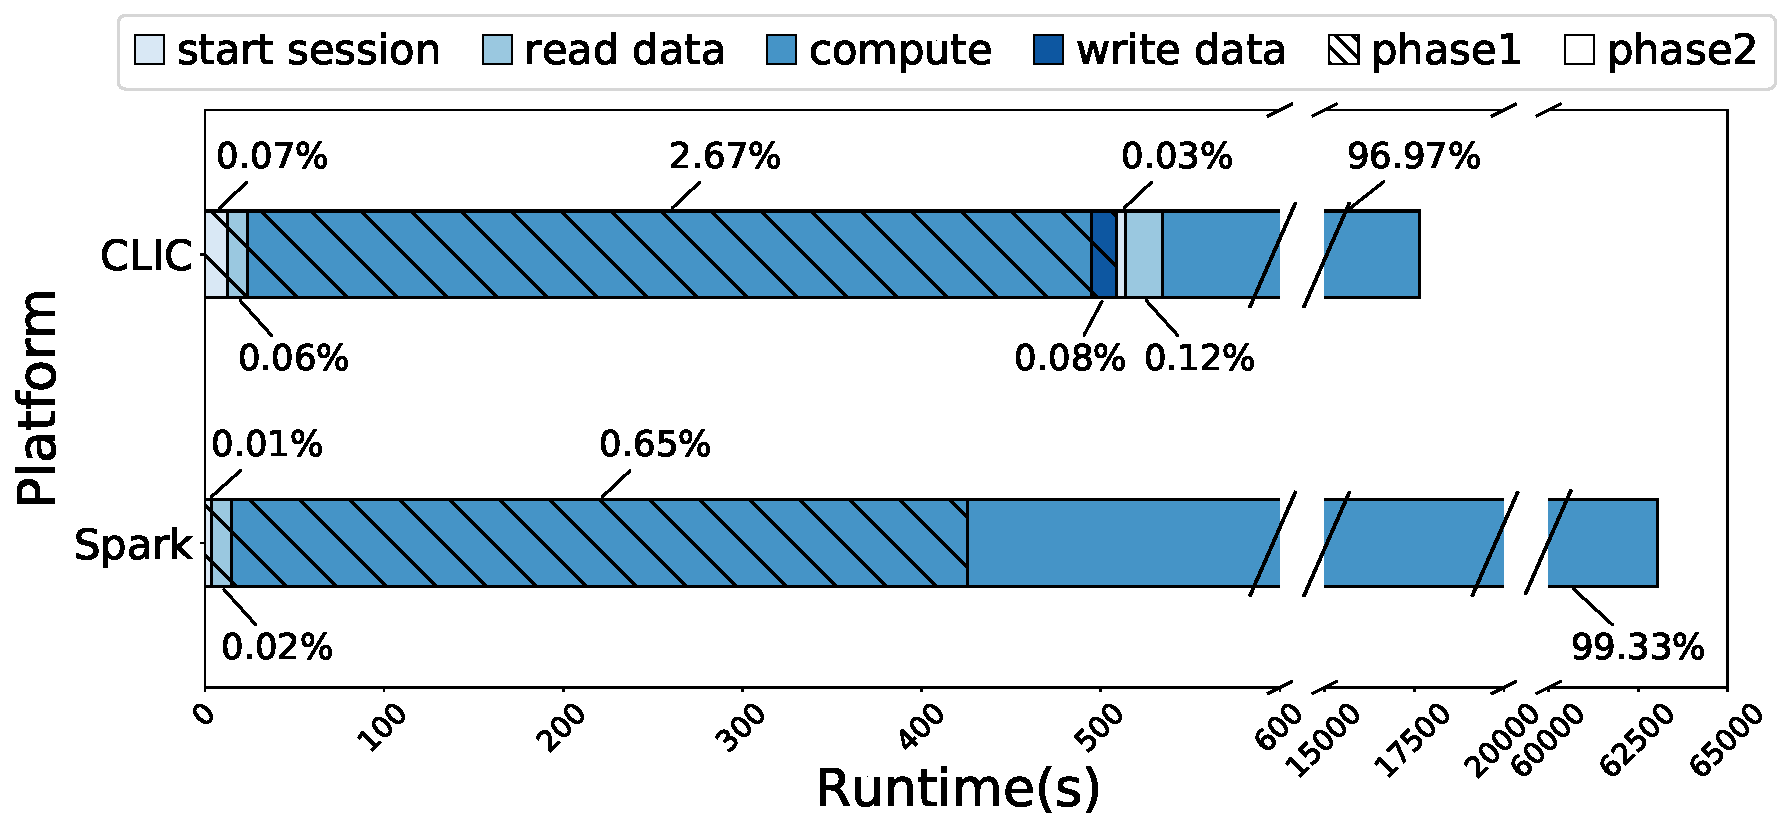
\includegraphics[width=0.8 \linewidth]{figures/chp6-nlp.pdf}
  \label{fig:hetero-nlp}
  }
  \subfigure[PageRank on Twitter Follower Network]{
  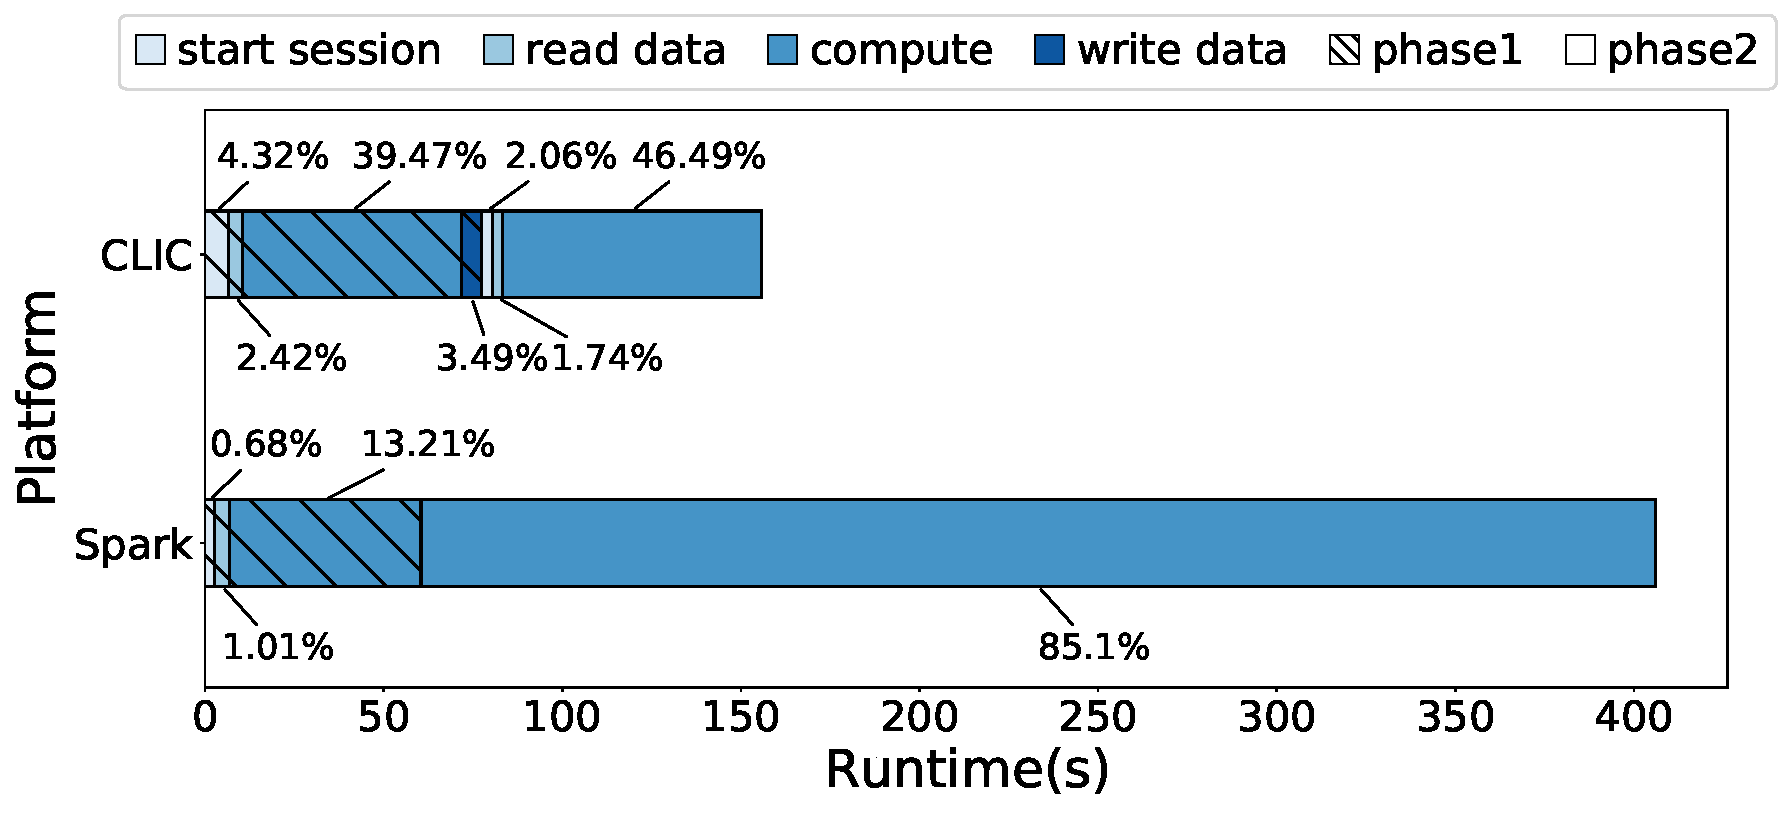
\includegraphics[width=0.8 \linewidth]{figures/chp6-pr-workflow.pdf}
  \label{fig:hetero-pr}
  }
  \caption{Performance comparison of two workflows}
  \label{fig:hetero}
\end{figure}

We consider two real-world workflows to validate CLIC’s ability to execute the workflow that contains multiple algebras. We record the time consumption of each stage when executing the workflow, including start session, data I/O, and computation.

The first workflow is the Sentiment Classification we have discussed in Section 3. It first reads and joins the two corpora using batch processing, which we call this \textit{phase1}, and then trains the deep learning model, which we call this \textit{phase2}. The training dataset is the Amazon Reviews\footnote{https://www.kaggle.com/bittlingmayer/amazonreviews} that consists of 3.4 million Amazon customer reviews (input text) and star ratings (output labels). Consider that Spark ML currently only supports a few simple machine learning models, we replace the LSTM~\cite{hochreiter1997long} with MLP (Multilayer Perception) for a fair comparison. As shown in Figure \ref{fig:hetero-nlp}, CLIC trains 3.6$\times$ faster than Spark. This is because CLIC migrates the model training process to the PyTorch platform that can use GPU for parallel training, therefore greatly reducing the training time, while the CPU-based Spark cannot obtain this benefit. Although the migration needs to read and write intermediate results across platforms, it can be seen from the percentage that its overhead is far less than the benefit from GPU acceleration. Moreover, both platforms achieve 78\% training accuracy. With the LSTM model, however, CLIC can achieve an accuracy of 97\%.

The second workflow is to perform PageRank on the Twitter follower network\footnote{https://snap.stanford.edu/data/twitter-2010.html}. It consists of extracting and filtering users who follow less than five other users (batch processing), constructing the graph, and performing PageRank (graph computing). We call the first procedure as \textit{phase1} and the last two procedures as \textit{phase2}. CLIC keeps the \textit{phase1} in Spark and migrates the phase2 to Giraph. The running time comparison between Spark and CLIC is shown in Figure \ref{fig:hetero-pr}, where the performance improvement brought by Giraph is significant comparing to the extra data movement overhead; therefore, CLIC finally demonstrates 4.8$\times$ performance improvement.

When processing data on two platforms, intermediate results need to be written from the first one and read by the following one. As shown in Figure~\ref{fig:hetero}, these overhead takes around 0.23\% and 7.29\% of the overall execution time. For the two workflows, launching tasks as containers on the cloud takes 0.07\% and 4.32\% of the execution time, respectively. Considering the performance improvements from cross-platform computing, these extra overhead is negligible. 
%We can conclude from the above two experiments that CLIC can not only execute the workflow that contains multiple algebras but also improve performance by utilizing different platforms properly.



\section{Conclusion}
We have made a strong case by designing and implementing CLIC to serve as a cloud-native framework for cross-platform workflows. Optimized for data science applications, CLIC supports agile platform integration, environment management, and flexible scaling. Experimental results on multiple platforms and applications show that CLIC is capable of selecting appropriate platforms for a workflow and enhancing its overall performance. Overall, CLIC demonstrates a promising solution for adopting cross-platform computing in building data science applications. 


\bibliographystyle{ACM-Reference-Format}
\bibliography{ref}

\end{document}
\endinput